\chapter{Confidence Intervals}
\label{ch:confidence-intervals}

\begin{chaptergoals}
\begin{itemize}[nosep]
\item What a confidence interval is: a \textit{random} interval, computable from the data alone, that traps the fixed parameter with a guaranteed probability. The two words that carry the definition are `random' and `computable'.
\item The recipe that produces every interval in this book: find a pivot (a quantity whose distribution you know), trap it between two quantiles, solve for the parameter. An exact pivot gives an exact interval; the CLT gives an asymptotic one.
\item Three ways around a pivot whose scale involves the unknown parameter: conservative, solve, plug-in. One picture explains all three and shows how they nest.
\item What drives the width (the level, through a quantile; the sample size, through $1/\sqrt{n}$), and what the $95\%$ does and does not mean.
\end{itemize}
The running examples are the kiss experiment ($n = 124$, $\bar{R}_n = 0.645$), for which \cref{ch:kiss} promised the interval $[0.56, 0.73]$, and the subway inter-arrival times of \cref{ch:limit-tools} ($n = 64$, $\bar{T}_n = 6.23$).
\end{chaptergoals}

\section{What a confidence interval is}
\label{sec:ci-definition}

\Cref{ch:estimators} produced a number, $\hat{p} = 0.645$, and a sampling distribution around it.
A confidence interval converts the two into a statement with a guarantee: a range of values of $p$, and a probability that the range is right.

\begin{definition}[Confidence interval]
\label{def:ci}
Let $\statmodel$ be a statistical model based on observations $\Xton$, with $\Theta \subseteq \real$, and let $\alpha \in (0,1)$.

A \textbf{confidence interval of level $1 - \alpha$} for $\theta$ is a random interval $\mathcal{I} = [L(\Xton), \, U(\Xton)]$ whose endpoints are statistics (their formulas don't involve $\theta$), such that
\[
\Pr_\theta \left( \mathcal{I} \ni \theta \right) \geq 1 - \alpha \quad \text{for all } \theta \in \Theta.
\]

A confidence interval of \textbf{asymptotic level $1 - \alpha$} is a random interval $\mathcal{I} = \mathcal{I}_n$ of the same kind such that
\[
\limn \Pr_\theta \left( \mathcal{I}_n \ni \theta \right) \geq 1 - \alpha \quad \text{for all } \theta \in \Theta.
\]
\end{definition}

\begin{inwords}
\textbf{In words.} A rule that turns a sample into an interval, computable from the sample alone, such that the interval it produces contains the true parameter at least $100(1 - \alpha)\%$ of the time, whatever the true parameter is. `Asymptotic' means the guarantee holds in the limit of large samples.
\par\smallskip
\textbf{For the kiss data.} The rule `$\bar{R}_n \pm 1.96\sqrt{\bar{R}_n(1 - \bar{R}_n)/n}$' is a confidence interval of asymptotic level $95\%$; on this sample it produced $[0.56, 0.73]$. The rule `$\bar{R}_n \pm 1.96\sqrt{p(1-p)/n}$' is not one, since $p$ is in its formula.
\end{inwords}

The notation $\mathcal{I} \ni \theta$ says `$\mathcal{I}$ contains $\theta$'.
It means the same as $\theta \in \mathcal{I}$, and this book writes it backwards on purpose: the random object, the thing the probability is about, is the interval on the left, not the parameter on the right.
Both appearances of $\theta$ in $\Pr_\theta(\mathcal{I} \ni \theta)$ are the same fixed number doing two jobs: as the subscript it fixes which distribution the sample is drawn from, and inside the parentheses it is the target that the interval either contains or misses.
Nothing in the expression is random except $\mathcal{I}$.

Three things in the definition deserve a second look.

\begin{enumerate}[nosep]
\item \textit{The interval is random; the parameter is not.} $L$ and $U$ are functions of the sample, so they're random variables, and $\mathcal{I}$ moves from sample to sample. $\theta$ is a fixed number that doesn't move. The probability is the probability that the moving interval lands on the fixed point.
\item \textit{The endpoints must be computable.} An interval whose formula contains $\theta$ is not a confidence interval, however nice its coverage probability: you can't compute it. This clause is what the three `solutions' of \cref{sec:ci-three-solutions} are solutions to.
\item \textit{The guarantee holds for every $\theta$.} You don't know $\theta$, so a guarantee that holds for some values of it and not others is no guarantee. This clause is what makes one of the intervals in \cref{ex:ci-fifty} fail.
\end{enumerate}

The inequality $\geq 1 - \alpha$ has a consequence worth stating once: a confidence interval of level $95\%$ is also a confidence interval of level $90\%$, of level $50\%$, of any level below $95\%$.
It is not, in general, one of level $98\%$.
`Level' is a floor on the coverage, not its exact value.

The word `level' is used for tests too (\cref{ch:tests-foundations}), where it denotes $\alpha$, the probability of rejecting a true hypothesis; for an interval the level is $1 - \alpha$, the probability of a correct capture.
Same $\alpha$, complementary conventions, and the context always says which is meant.

\begin{intuition}[a procedure, not a number]
The confidence interval is the \textit{rule} that turns a sample into an interval, $(x_1, \ldots, x_n) \mapsto [L, U]$, and the level is a property of the rule: the fraction of samples on which the rule's output contains $\theta$.
Once you apply the rule to your one sample you get two numbers, $[0.56, 0.73]$.
Those numbers are not random and the parameter is not random, so the pair has no probability attached: $[0.56, 0.73]$ either contains $p$ or it doesn't, and you will never know which.
What you know is that the rule that produced it is right $95\%$ of the time.
\Cref{fig:cirepeated} is this sentence as a picture.
The kiss experiment was simulated $100$ times with $n = 124$ and $p = 0.645$, and the plug-in interval of \cref{sec:ci-three-solutions} was computed each time.
The parameter is the fixed vertical line; the intervals move, and each is centered at its own $\hat{p}$.
Sorted by $\hat{p}$, the six that miss are the samples whose proportion came out unusually low or high.
Ninety-four of the hundred contain $0.645$ and six don't, and the level $95\%$ is the long-run rate of the first kind, not a statement about any one of the hundred intervals.
\end{intuition}

\begin{figure}[htbp]
\centering
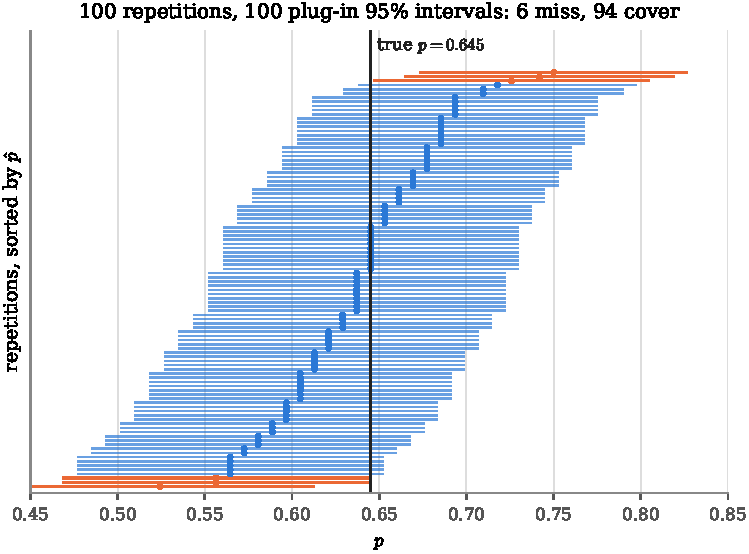
\includegraphics[width=\textwidth]{fig_ci_repeated}
\caption{One hundred simulated kiss experiments with $n = 124$ and $p = 0.645$, sorted by $\hat{p}$ (dot), each with its $95\%$ plug-in interval. The black vertical line is $p$; intervals that contain it are blue, the six that miss are orange.}
\label{fig:cirepeated}
\end{figure}

\section{The recipe, on an exact case}
\label{sec:ci-recipe}

Every interval in this book is built the same way, and the cleanest place to see the construction is the one case where nothing is asymptotic.

\begin{worked}[Gaussian data, known variance]
Let $\Xton \iid \Gauss(\mu, \sigma^2)$ with $\sigma^2$ known and $\mu$ unknown.
By \cref{ch:gaussian}, $\bar{X}_n \sim \Gauss(\mu, \sigma^2/n)$ exactly, for every $n$, so
\[
Z = \sqrt{n} \, \frac{\bar{X}_n - \mu}{\sigma} \sim \Gauss(0, 1) \quad \text{for every } n \text{ and every } \mu.
\]
A quantity like $Z$, a function of the data and the parameter whose distribution doesn't depend on the parameter, is called a \textbf{pivot}.
The recipe has three steps.
\begin{enumerate}[nosep]
\item \textit{Trap the pivot.} With $q_{\alpha/2}$ the quantile of \cref{sec:gauss-quantiles}, $\Pr(-q_{\alpha/2} \leq Z \leq q_{\alpha/2}) = 1 - \alpha$.
\item \textit{Rewrite the event.} $-q_{\alpha/2} \leq \sqrt{n}(\bar{X}_n - \mu)/\sigma \leq q_{\alpha/2}$ is the same event as $\abs{\bar{X}_n - \mu} \leq q_{\alpha/2} \, \sigma/\sqrt{n}$.
\item \textit{Solve for the parameter.} That event is the same as
\[
\mu \in \left[ \bar{X}_n - q_{\alpha/2} \frac{\sigma}{\sqrt{n}}, \; \bar{X}_n + q_{\alpha/2} \frac{\sigma}{\sqrt{n}} \right] =: \mathcal{I}.
\]
\end{enumerate}
The event in step 3 is the event in step 1, written differently, so $\Pr_\mu(\mathcal{I} \ni \mu) = 1 - \alpha$ for every $\mu$ and every $n$.
The endpoints involve $\bar{X}_n$, $\sigma$ (known), $n$ and a quantile, none of which is $\mu$, so $\mathcal{I}$ is a confidence interval of level $1 - \alpha$, with no limit anywhere.
For $\alpha = 0.05$ it is $\bar{X}_n \pm 1.96 \, \sigma/\sqrt{n}$.
\end{worked}

\begin{bridge}[estimate $\pm$ margin of error]
The interval you learned is `point estimate $\pm$ (critical value) $\times$ (standard error)'.
The recipe says where each piece comes from: the point estimate is the center because the pivot is centered at the parameter; the critical value is the quantile that traps the pivot; the standard error is the pivot's scale, $\sigma/\sqrt{n}$.
When $\sigma$ is unknown, an introductory course replaces it by $s$ and switches to a $t$ critical value: that is a different pivot, $\sqrt{n}(\bar{X}_n - \mu)/s$, with an exact Student distribution for Gaussian data, and \cref{ch:t-test} derives it.
For large $n$ and any parent distribution, the replacement is justified by Slutsky instead (\cref{sec:slutsky}), which is the route this chapter takes.
\end{bridge}

\textbf{One-sided intervals.}
Nothing forces step 1 to trap the pivot symmetrically.
$\Pr(Z \leq q_\alpha) = 1 - \alpha$ as well, and solving $\sqrt{n}(\bar{X}_n - \mu)/\sigma \leq q_\alpha$ for $\mu$ gives
\[
\mu \in \left[ \bar{X}_n - q_\alpha \frac{\sigma}{\sqrt{n}}, \; \infty \right),
\]
a \textbf{lower confidence bound}: `$\mu$ is at least this much', with level $1 - \alpha$.
Trapping $Z \geq -q_\alpha$ gives the upper bound $(-\infty, \bar{X}_n + q_\alpha \sigma/\sqrt{n}]$.
Note the quantile: $q_\alpha$ ($1.645$ at $95\%$), not $q_{\alpha/2}$ ($1.96$) because all of the $5\%$ of misses is spent on one side.
One-sided intervals are the confidence-interval face of one-sided tests, and \cref{ex:ci-onesided} makes the correspondence exact.

\section{The kiss experiment: an interval that isn't one}
\label{sec:ci-kiss-problem}

Now $R_1, \ldots, R_n \iid \Bern(p)$, $\hat{p} = \bar{R}_n$, and there is no exact pivot in sight: the distribution of $\bar{R}_n$ is Binomial, scaled, and it depends on $p$ in a way that no simple transformation removes.
What there is instead is the CLT (\cref{thm:clt}).
\recall{The Central Limit Theorem says that the error of an average, magnified by $\sqrt{n}$ and divided by the standard deviation of one observation, has a distribution that settles down to $\Gauss(0,1)$, whatever the observations were drawn from. You do not need to know that distribution to use the theorem; you need only its mean and variance.}
\[
\sqrt{n} \, \frac{\bar{R}_n - p}{\sqrt{p(1-p)}} \convd \Gauss(0, 1).
\]
The left side is an \textit{asymptotic} pivot: its distribution depends on $p$ for every finite $n$, but its limit doesn't.
Convergence in distribution means convergence of the CDF at every continuity point of the limit (\cref{sec:conv-dist}), and the Gaussian CDF is continuous everywhere, so
\[
\limn \Pr_p \left( -q_{\alpha/2} \leq \sqrt{n} \, \frac{\bar{R}_n - p}{\sqrt{p(1-p)}} \leq q_{\alpha/2} \right) = \Pr(-q_{\alpha/2} \leq Z \leq q_{\alpha/2}) = 1 - \alpha.
\]
Steps 2 and 3 of the recipe then give
\begin{equation}
\label{eq:ci-not-a-ci}
\limn \Pr_p \left( \left[ \bar{R}_n - q_{\alpha/2} \sqrt{\frac{p(1-p)}{n}}, \; \bar{R}_n + q_{\alpha/2} \sqrt{\frac{p(1-p)}{n}} \right] \ni p \right) = 1 - \alpha.
\end{equation}
This looks like the Gaussian case with $\sigma$ replaced by $\sqrt{p(1-p)}$, and it has the right asymptotic coverage, \textit{but it is not a confidence interval}: the endpoints contain $p$.
You can't compute $\bar{R}_n \pm 1.96 \sqrt{p(1-p)/124}$ without knowing the thing you're estimating.
The pivot's scale depends on the parameter, and the recipe's step 3 is stuck.

\begin{figure}[htbp]
\centering
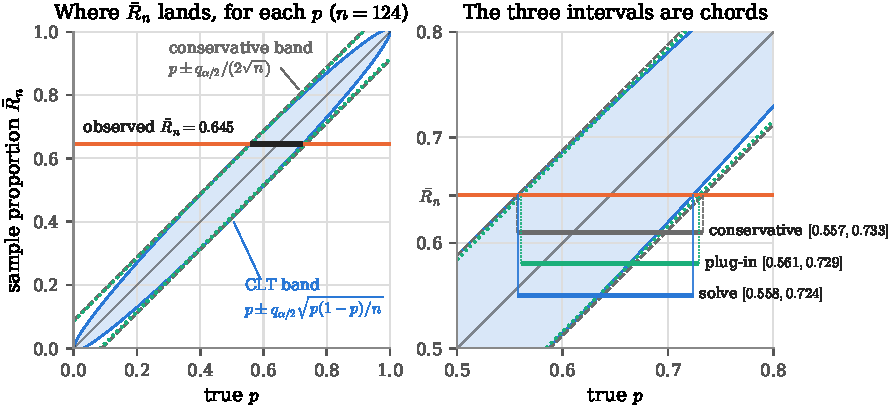
\includegraphics[width=\textwidth]{fig_ci_inversion}
\caption{Sample proportion against the true $p$, $n = 124$. Left: the CLT band $p \pm q_{\alpha/2}\sqrt{p(1-p)/n}$ (blue), the widest band (gray dashes), a band of constant width (aqua dots) and the observed $\bar{R}_n = 0.645$ (orange line). Right: the three chords, to scale.}
\label{fig:ciinversion}
\end{figure}

\section{Three ways to get unstuck}
\label{sec:ci-three-solutions}

\Cref{fig:ciinversion} is the picture to hold on to.
For each candidate value of $p$ on the horizontal axis, the CLT band is the set of sample proportions that value would plausibly produce: by \cref{eq:ci-not-a-ci}, $\bar{R}_n$ lands in $p \pm q_{\alpha/2}\sqrt{p(1-p)/n}$ about $95\%$ of the time, and the band is a lens, widest at $p = \frac12$ and pinched at the ends.
Reading the picture downwards, from a $p$ to its band, is probability.
Reading it sideways, from the observed $\bar{R}_n = 0.645$ (the horizontal line) to the set of $p$ whose bands reach it, is statistics, and that set is the confidence interval.
With the lens itself, it is the chord the line cuts out of the lens, and that chord is the solve interval.
The three solutions differ in which band they read.
The conservative interval replaces the lens by the widest band it fits in, and gets a longer chord.
The plug-in interval replaces the lens by a band of constant width $q_{\alpha/2}\sqrt{\hat{p}(1-\hat{p})/n}$, the width the lens has at $p = \hat{p}$, and gets a chord of nearly the same length, centered at $\hat{p}$.
The right of the figure shows the three chords to scale, with $n = 124$.

\subsection*{Solution 1: conservative}

Whatever $p$ is, $p(1-p) \leq \frac14$, with equality at $p = \frac12$.
So the event in \cref{eq:ci-not-a-ci} is contained in a larger event with a computable boundary:
\[
\abs{\bar{R}_n - p} \leq q_{\alpha/2} \sqrt{\frac{p(1-p)}{n}} \quad \Longrightarrow \quad \abs{\bar{R}_n - p} \leq \frac{q_{\alpha/2}}{2\sqrt{n}}.
\]
Define
\[
\mathcal{I}_{\text{conserv}} = \left[ \bar{R}_n - \frac{q_{\alpha/2}}{2\sqrt{n}}, \; \bar{R}_n + \frac{q_{\alpha/2}}{2\sqrt{n}} \right].
\]
Its coverage is at least that of the CLT event, so $\limn \Pr_p(\mathcal{I}_{\text{conserv}} \ni p) \geq 1 - \alpha$ for every $p$: an asymptotic confidence interval, with the inequality of the definition used in earnest.
The coverage is exactly $1 - \alpha$ in the limit only at $p = \frac12$; elsewhere the interval is wider than it needs to be, which is what `conservative' means.
In the figure it reads the widest band instead of the lens.

With $n = 124$: $q_{0.025}/(2\sqrt{124}) = 1.96/22.27 = 0.088$, so $\mathcal{I}_{\text{conserv}} = [0.557, 0.733]$.

\subsection*{Solution 2: solve}

Keep the lens and do step 3 properly.
The event $\abs{\bar{R}_n - p} \leq q_{\alpha/2}\sqrt{p(1-p)/n}$ is, after squaring,
\[
(\bar{R}_n - p)^2 \leq \frac{q_{\alpha/2}^2}{n} \, p(1-p),
\qquad \text{that is,} \qquad
\left( 1 + \frac{q_{\alpha/2}^2}{n} \right) p^2 - \left( 2\bar{R}_n + \frac{q_{\alpha/2}^2}{n} \right) p + \bar{R}_n^2 \leq 0.
\]
The left side is a convex quadratic in $p$, so the inequality holds exactly between its two roots $p_1 < p_2$, and
\[
\mathcal{I}_{\text{solve}} = [p_1, p_2]
\]
is the \textit{same event} as the one in \cref{eq:ci-not-a-ci}, now with computable endpoints: $\limn \Pr_p(\mathcal{I}_{\text{solve}} \ni p) = 1 - \alpha$, with equality.
The quadratic formula gives the roots in closed form,
\begin{equation}
\label{eq:wilson}
p_{1,2} = \frac{1}{1 + q_{\alpha/2}^2/n} \left( \bar{R}_n + \frac{q_{\alpha/2}^2}{2n} \; \mp \; q_{\alpha/2} \sqrt{ \frac{\bar{R}_n(1 - \bar{R}_n)}{n} + \frac{q_{\alpha/2}^2}{4n^2} } \right),
\end{equation}
an interval known as the Wilson score interval.
The word `score' is explained in \cref{sec:tests-duality}: this interval is what you get by inverting a standard test of $H_0: p = p_0$, the score test, which measures distance from $p_0$ in units of the standard error computed at $p_0$.
Note that it is \textit{not} centered at $\bar{R}_n$: its center is pulled toward $\frac12$, by an amount of order $1/n$ because the lens is wider there.

With $n = 124$, $\bar{R}_n = 80/124$ and $q_{0.025} = 1.96$ the quadratic is $1.0310\,p^2 - 1.3213\,p + 0.4162 \leq 0$, with roots $p_1 = 0.558$ and $p_2 = 0.724$: $\mathcal{I}_{\text{solve}} = [0.558, 0.724]$.

\begin{pitfall}[rounding the quadratic before solving it]
Solve for $p_1$ and $p_2$ from the coefficients as computed, not from rounded versions of them.
A quadratic's roots are sensitive to its coefficients, and this quadratic is a bad case.
Its constant term is $0.4162$; carrying that to two decimals as $0.41$ moves the roots three points each way, to $[0.53, 0.75]$, and rounding it up to $0.42$ instead gives $[0.59, 0.69]$, wrong in the other direction.
Two decimals are not enough here either way, and the error is large enough to change the conclusion: the $[0.53, 0.75]$ that the truncated coefficients produce is wider than the conservative interval $[0.557, 0.733]$, while the true solve interval $[0.558, 0.724]$ is the narrowest of the three.
The solve interval can never be the widest, since \cref{prop:ci-nesting} shows it always sits inside the conservative interval, so an interval that comes out wider than the conservative one is an arithmetic error and nothing else.
\end{pitfall}

\subsection*{Solution 3: plug-in}

Replace the unknown scale $\sqrt{p(1-p)}$ by its estimate $\sqrt{\hat{p}(1 - \hat{p})}$, and let Slutsky's theorem pay for it.
\recall{Slutsky's theorem is the rule that lets you substitute an estimate for an unknown constant inside a limit: if one quantity settles into a distribution and a second converges in probability to a constant, their product and their sum behave as if the second simply \textit{were} that constant. It is what makes every `estimate $\pm$ standard error' formula legitimate.}
This is the worked example of \cref{sec:slutsky}: since $\hat{p} \convp p$ (LLN) and $x \mapsto \sqrt{p(1-p)/(x(1-x))}$ is continuous at $p$ (CMT),
\[
\sqrt{n} \, \frac{\bar{R}_n - p}{\sqrt{\hat{p}(1 - \hat{p})}}
= \underbrace{\sqrt{n} \, \frac{\bar{R}_n - p}{\sqrt{p(1-p)}}}_{\convd \Gauss(0,1)} \cdot \underbrace{\sqrt{\frac{p(1-p)}{\hat{p}(1-\hat{p})}}}_{\convp 1} \convd \Gauss(0,1).
\]
The left side is a new asymptotic pivot whose scale no longer involves $p$, so the recipe runs to the end:
\[
\mathcal{I}_{\text{plug-in}} = \left[ \bar{R}_n - q_{\alpha/2} \sqrt{\frac{\hat{p}(1-\hat{p})}{n}}, \; \bar{R}_n + q_{\alpha/2} \sqrt{\frac{\hat{p}(1-\hat{p})}{n}} \right],
\qquad \limn \Pr_p(\mathcal{I}_{\text{plug-in}} \ni p) = 1 - \alpha.
\]
In the figure it reads a band of constant width, the lens's width at $\hat{p}$.
The price is a second asymptotic approximation on top of the CLT: Slutsky's theorem is a statement about $n \to \infty$, and at finite $n$ the estimated scale is itself noisy.

With $n = 124$: $1.96 \sqrt{0.645 \times 0.355/124} = 0.084$, so $\mathcal{I}_{\text{plug-in}} = [0.561, 0.729]$.

\subsection*{The three side by side}

\begin{center}
\begin{tabular}{@{}ll>{\raggedright\arraybackslash}p{3.6cm}>{\raggedright\arraybackslash}p{4.6cm}@{}}
\toprule
Interval & $95\%$, $n = 124$ & Reads & Asymptotic coverage \\
\midrule
conservative & $[0.557, 0.733]$ & the widest band & $\geq 1 - \alpha$; $= 1 - \alpha$ only at $p = \frac12$ \\[2pt]
solve & $[0.558, 0.724]$ & the lens itself & $= 1 - \alpha$; one approximation (CLT) \\[2pt]
plug-in & $[0.561, 0.729]$ & a band of half-width $q_{\alpha/2}\sqrt{\hat{p}(1-\hat{p})/n}$ & $= 1 - \alpha$; two approximations (CLT, Slutsky) \\
\bottomrule
\end{tabular}
\end{center}

The conservative and plug-in intervals round to the $[0.56, 0.73]$ that \cref{ch:kiss} promised, the solve interval to $[0.56, 0.72]$, and \cref{ch:kiss}'s drug example is the same computation: $78$ of $100$ cured gives $\hat{p} = 0.78$ and $\mathcal{I}_{\text{plug-in}} = 0.78 \pm 1.96\sqrt{0.78 \times 0.22/100} = [0.699, 0.861]$, the $[0.70, 0.86]$ quoted there.
There are more intervals still; the exact interval built from the Binomial distribution of $n\bar{R}_n$ rather than from the CLT (the Clopper--Pearson interval mentioned in \cref{sec:conv-what-limits-buy}) gives $[0.554, 0.729]$ for the kiss data, and Newcombe (1998) compares seven of them on coverage and width.\footnote{R.\ Newcombe, `Two-sided confidence intervals for the single proportion: comparison of seven methods', \textit{Statistics in Medicine} 17 (1998).}
That they all agree to within a point is the CLT doing its job at $n = 124$.

\begin{proposition}[How the three nest]
\label{prop:ci-nesting}
For every sample and every $n$: $\mathcal{I}_{\text{solve}} \subseteq \mathcal{I}_{\text{conserv}}$ and $\mathcal{I}_{\text{plug-in}} \subseteq \mathcal{I}_{\text{conserv}}$, and both $\mathcal{I}_{\text{solve}}$ and $\mathcal{I}_{\text{plug-in}}$ contain $\bar{R}_n$.
\end{proposition}
\coreproof{Everything follows from $p(1-p) \leq \frac14$: a $p$ that passes the solve test passes the conservative one, and the plug-in half-width is at most the conservative half-width.}
\begin{proof}
If $p \in \mathcal{I}_{\text{solve}}$ then $\abs{\bar{R}_n - p} \leq q_{\alpha/2}\sqrt{p(1-p)/n} \leq q_{\alpha/2}/(2\sqrt{n})$, so $p \in \mathcal{I}_{\text{conserv}}$.
The plug-in half-width is $q_{\alpha/2}\sqrt{\hat{p}(1-\hat{p})/n} \leq q_{\alpha/2}/(2\sqrt{n})$, the conservative one.
Finally $p = \bar{R}_n$ satisfies the solve inequality trivially ($0 \leq$ something non-negative), and the plug-in interval is centered there.
\end{proof}

In the picture: the lens lies inside the widest band, so any chord of the lens lies inside the corresponding chord of the band.
Solve and plug-in need not nest with each other; here the solve interval is shifted toward $\frac12$ and slightly shorter.

\begin{intuition}[which one to use]
Use the solve interval for a proportion, the plug-in interval for everything else.
The defense: the solve interval has the exact asymptotic level with one approximation, has a closed form (\cref{eq:wilson}) and, as \cref{fig:cicoverage} shows, holds up at finite $n$ far better than the plug-in interval near $p = 0$ or $1$, where the latter breaks; the only reason it isn't universal is that `solve for the parameter' is a quadratic here and may be intractable elsewhere.
The plug-in interval is the one every formula sheet gives, is what the next chapters use, and is fine whenever $n\hat{p}(1-\hat{p})$ is comfortably large; \cref{ch:wald-lrt} identifies it as an inverted Wald test and, for models other than the proportion, recommends the likelihood ratio interval in its place.
The conservative interval is for two jobs: a guaranteed level, and planning sample sizes before any data exist (\cref{sec:ci-width}), since it is the only one of the three whose width you know in advance.
\end{intuition}

\section{What `asymptotic level' buys at a finite \texorpdfstring{$n$}{n}}
\label{sec:ci-coverage}

Asymptotic level $1 - \alpha$ is a promise about $n \to \infty$.
For a proportion you can check what it delivers at the $n$ you have because the distribution of $n\bar{R}_n$ is Binomial and the coverage probability is a finite sum:
\[
\Pr_p(\mathcal{I} \ni p) = \sum_{k=0}^{n} \binom{n}{k} p^k (1-p)^{n-k} \, \ind\big( \mathcal{I}(k) \ni p \big),
\]
where $\mathcal{I}(k)$ is the interval the rule produces when $k$ of the $n$ couples turn right.
\Cref{fig:cicoverage} plots this against $p$ for the three intervals, at $n = 124$ and at $n = 20$.
The conservative interval over-covers away from $p = \frac12$: its coverage is $0.99995$ at $p = 0.05$.
The plug-in interval under-covers, mildly at $n = 124$ ($0.939$ at $p = 0.645$) and badly at $n = 20$ near the edges.
The solve interval stays near $0.95$ at $n = 124$ ($0.952$ at $p = 0.645$) and above $0.92$ at $n = 20$ for $p$ between $0.01$ and $0.99$, where the plug-in interval falls as low as $0.33$, below the bottom of the plot.
The saw teeth are real, not noise: $\bar{R}_n$ takes only $n + 1$ values, so there are only $n + 1$ possible intervals, and the coverage jumps whenever $p$ crosses an endpoint of one of them.

\begin{figure}[htbp]
\centering
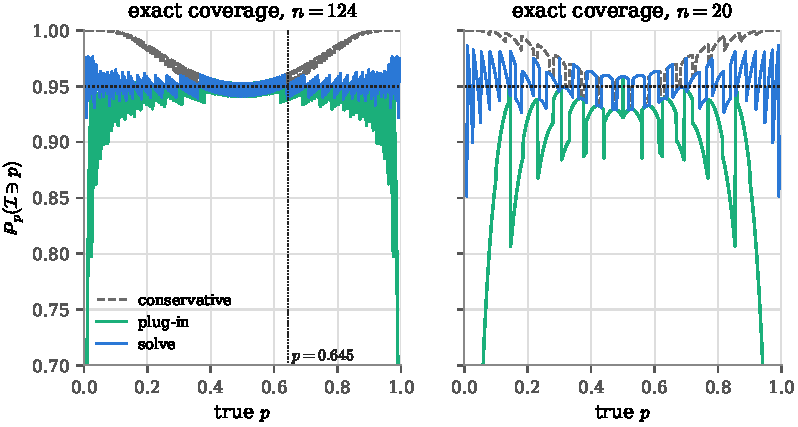
\includegraphics[width=\textwidth]{fig_ci_coverage}
\caption{Exact coverage probability $\Pr_p(\mathcal{I} \ni p)$ of the three $95\%$ intervals against the true $p$: conservative (gray dashes), plug-in (aqua) and solve (blue), with the nominal $0.95$ as a dotted line. Left, $n = 124$; right, $n = 20$.}
\label{fig:cicoverage}
\end{figure}

Three lessons from the figure.
The asymptotic promise is kept at $n = 124$ to within a point or two for $p$ in the middle of $(0,1)$, which is where the kiss data put it.
The plug-in interval is the one that fails first as $n$ shrinks or $p$ approaches the edges because its width is $\sqrt{\hat{p}(1-\hat{p})/n}$ and $\hat{p}$ near $0$ or $1$ makes it think it is very precise (at $\hat{p} = 0$ its width is zero).
And the conservative interval is not free: its extra width buys coverage you didn't ask for, and that over-coverage is wasted precision.

This is the chapter's instance of the book's stance on asymptotics (the intuition box that opens \cref{ch:lln}, and \cref{sec:conv-what-limits-buy}): the theorem licenses the Gaussian replacement and is silent about the error at your $n$.
For a proportion the error can be computed, as here.
For most models it can't, and the plug-in interval is used on trust and on the experience that $n$ in the dozens with a parameter away from the boundary is usually enough.

\section{The subway: when the scale depends on the parameter in a new way}
\label{sec:ci-subway}

The three solutions were introduced for a proportion, where the scale $\sqrt{p(1-p)}$ is bounded.
The inter-arrival-time example of \cref{sec:delta-method} shows what changes when it isn't.
$T_1, \ldots, T_n \iid \Expo(\lambda)$, $\hat{\lambda} = 1/\bar{T}_n$, and the delta method gave
\recall{The delta method says what happens to a transformed estimator: if $\hat\theta_n$ is approximately Gaussian around $\theta$ with standard deviation $\sigma/\sqrt{n}$, then $g(\hat\theta_n)$ is approximately Gaussian around $g(\theta)$ with standard deviation $\abs{g'(\theta)}\sigma/\sqrt{n}$. The slope of $g$ at $\theta$ stretches or compresses the error.}
\[
\sqrt{n} \, (\hat{\lambda} - \lambda) \convd \Gauss(0, \lambda^2),
\qquad \text{so} \qquad
\limn \Pr_\lambda \left( \abs{\hat{\lambda} - \lambda} \leq q_{\alpha/2} \frac{\lambda}{\sqrt{n}} \right) = 1 - \alpha.
\]
Again the half-width involves the parameter, now as a factor $\lambda$ rather than $\sqrt{p(1-p)}$, and \cref{fig:ciwedge} shows the consequence: the band is a wedge, not a lens.
For each true $\lambda$, the delta method says $\hat{\lambda}$ lands in $\lambda \pm q_{\alpha/2}\lambda/\sqrt{n}$ about $95\%$ of the time, and that band keeps opening as $\lambda$ grows, with no widest point.
The observed $\hat{\lambda} = 1/6.23 = 0.1605$ is the horizontal line, and the solve interval is the chord it cuts from the wedge, which is not centered at $\hat{\lambda}$ because the wedge is wider to the right.
The plug-in interval uses a band of constant width $q_{\alpha/2}\hat{\lambda}/\sqrt{n}$ and is centered.
No band of constant width contains the wedge, so there is nothing for a conservative interval to read.

\begin{figure}[htbp]
\centering
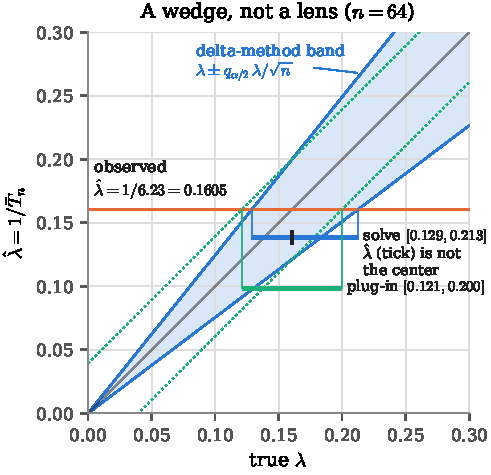
\includegraphics[width=0.62\textwidth]{fig_ci_wedge}
\caption{The subway rate, $n = 64$: $\hat{\lambda}$ against the true $\lambda$. The delta-method band $\lambda \pm q_{\alpha/2}\lambda/\sqrt{n}$ (blue), the plug-in band of constant width (aqua dots), the observed $\hat{\lambda} = 0.1605$ (orange line) and the two chords below it.}
\label{fig:ciwedge}
\end{figure}

\begin{enumerate}[nosep]
\item \textit{Conservative:} there is nothing to bound. $\lambda$ ranges over $(0, \infty)$, so $\sup_\lambda q_{\alpha/2}\lambda/\sqrt{n} = \infty$ and the `conservative interval' is $(0, \infty)$, which has level $100\%$ and says nothing.
\item \textit{Solve:} the inequality is linear in $\lambda$ this time. $\abs{\hat{\lambda} - \lambda} \leq q_{\alpha/2}\lambda/\sqrt{n}$ is the same as $\lambda(1 - q_{\alpha/2}/\sqrt{n}) \leq \hat{\lambda} \leq \lambda(1 + q_{\alpha/2}/\sqrt{n})$, and if $n > q_{\alpha/2}^2$ (so that $1 - q_{\alpha/2}/\sqrt{n} > 0$) this solves to
\[
\mathcal{I}_{\text{solve}} = \left[ \frac{\hat{\lambda}}{1 + q_{\alpha/2}/\sqrt{n}}, \; \frac{\hat{\lambda}}{1 - q_{\alpha/2}/\sqrt{n}} \right].
\]
\item \textit{Plug-in:} replace $\lambda$ in the half-width by $\hat{\lambda}$ (Slutsky, since $\hat{\lambda} \convp \lambda$):
\[
\mathcal{I}_{\text{plug-in}} = \left[ \hat{\lambda} \left( 1 - \frac{q_{\alpha/2}}{\sqrt{n}} \right), \; \hat{\lambda} \left( 1 + \frac{q_{\alpha/2}}{\sqrt{n}} \right) \right].
\]
\end{enumerate}
With $n = 64$ and $\bar{T}_n = 6.23$ minutes: $\hat{\lambda} = 0.1605$ per minute and $q_{0.025}/\sqrt{64} = 0.245$, so
\[
\mathcal{I}_{\text{solve}} = [0.129, 0.213] \approx [0.13, 0.21], \qquad \mathcal{I}_{\text{plug-in}} = [0.121, 0.200] \approx [0.12, 0.20].
\]
The two differ more than the kiss intervals did because $n = 64$ is smaller and $q/\sqrt{n} = 0.245$ is not small: $1/(1 - 0.245) = 1.32$ against $1 + 0.245 = 1.245$.
The solve interval reaches further to the right, where the wedge is wider: large values of $\lambda$ produce more variable $\hat{\lambda}$, so more of them are compatible with the observed $0.16$.

\begin{remark}
There is a second way to see the solve interval that explains its asymmetry.
Build the plug-in interval for the \textit{mean} $1/\lambda$ first: the CLT gives $\sqrt{n}(\bar{T}_n - 1/\lambda) \convd \Gauss(0, 1/\lambda^2)$, and plugging in gives $\bar{T}_n(1 \pm q_{\alpha/2}/\sqrt{n}) = [4.70, 7.76]$ minutes.
Now map it through $x \mapsto 1/x$, which is decreasing: $\lambda \in [1/7.76, 1/4.70] = [0.129, 0.213]$, which is $\mathcal{I}_{\text{solve}}$ exactly.
A confidence interval for $\theta$ becomes a confidence interval for $g(\theta)$, with the same level, by applying any continuous and strictly monotone $g$ to its endpoints, in the right order ($[g(L), g(U)]$ for increasing $g$, $[g(U), g(L)]$ for decreasing $g$) because $\theta \in [L, U]$ and $g(\theta) \in g([L, U])$ are the same event.
The delta method is needed when $g$ is not monotone (the odds of \cref{ch:limit-tools} are, $p(1-p)$ is not), or when you want the interval for $g(\theta)$ to be symmetric about $g(\ethn)$, and symmetry is not a virtue in itself.
\end{remark}

\section{What makes an interval wide}
\label{sec:ci-width}

The half-width of the conservative and plug-in intervals is exactly
\[
\text{half-width} = q_{\alpha/2} \times \frac{\widehat{\sigma}}{\sqrt{n}},
\]
a quantile times an estimated standard error, and the solve intervals have the same size up to terms of smaller order.
The two factors are the two things you control.

\begin{figure}[htbp]
\centering
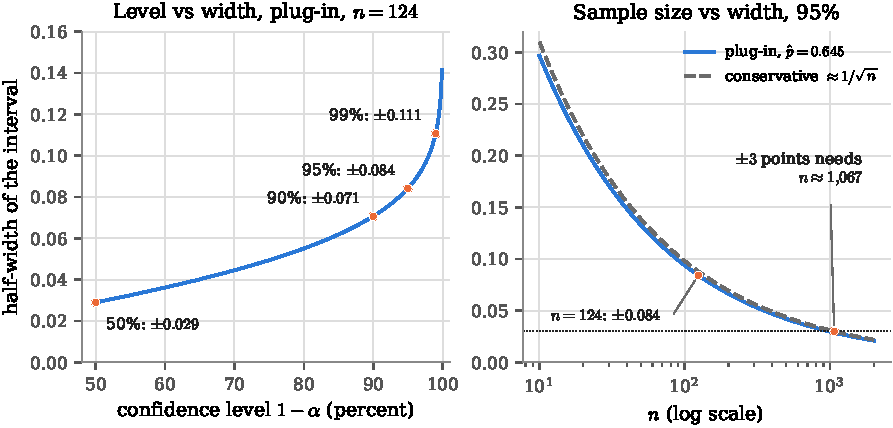
\includegraphics[width=\textwidth]{fig_ci_width}
\caption{Left: the half-width of the plug-in interval at $\hat{p} = 0.645$, $n = 124$, against the confidence level, with orange dots at the usual levels. Right: the half-width at $95\%$ against $n$, plug-in at $\hat{p} = 0.645$ (blue) and conservative (gray dashes).}
\label{fig:ciwidth}
\end{figure}

\textbf{The level.}
Raising the confidence level widens the interval, through the quantile, and the cost accelerates (\cref{fig:ciwidth}, left).
The quantile $q_{\alpha/2}$ does the work: $0.67$ at $50\%$, $1.645$ at $90\%$, $1.96$ at $95\%$, $2.58$ at $99\%$, $3.29$ at $99.9\%$, and infinite at $100\%$.
Going from $90\%$ to $95\%$ costs $19\%$ more width; from $95\%$ to $99\%$, $31\%$ more; and $100\%$ confidence costs the whole parameter space, since $q_{\alpha/2} \to \infty$ as $\alpha \to 0$.
This is why $95\%$ is a convention and not a law: it is a point on a curve where the interval is still informative and the miss rate is still small.
A $98\%$ interval of the same type always contains the $95\%$ one because $q_{0.01} > q_{0.025}$; but a $98\%$ interval need not contain a $95\%$ interval built differently. $[0, \, \bar{R}_n + q_{0.02}\,\widehat{\sigma}/\sqrt{n}]$ has asymptotic level $98\%$ and does not contain the $95\%$ lower-bound interval $[\bar{R}_n - q_{0.05}\,\widehat{\sigma}/\sqrt{n}, \, 1]$, nor the other way around: the $98\%$ interval reaches down to $0$ but stops short of $1$, the $95\%$ one reaches up to $1$ but stops short of $0$, so each contains points the other does not.
Nesting holds within one family of intervals indexed by $\alpha$, not between two intervals of different shapes whose levels happen to differ.

\textbf{The sample size.}
The width shrinks like $1/\sqrt{n}$ (\cref{fig:ciwidth}, right), which is the rate of the CLT and the rate of every interval in this book built from a sample mean.
Both curves on the right fall at that rate, the plug-in half-width at $\hat{p} = 0.645$ and the conservative half-width $q_{0.025}/(2\sqrt{n}) = 0.98/\sqrt{n}$, which is the pollster's `about $1/\sqrt{n}$'; the marked point is the $n \approx 1{,}067$ that a margin of $\pm 3$ points needs.
The practical form of $1/\sqrt{n}$: to halve the width you need four times the data; to get one more decimal place you need a hundred times the data.
Intervals that shrink faster exist when the model has special structure (\cref{ex:ci-shifted-expo} has one that shrinks like $1/n$), but they are built on the model's exact distribution rather than on the CLT, and they are fragile when the model is wrong.

\begin{bridge}[the pollster's $\pm 3$ points]
National polls report a `margin of error of $\pm 3$ percentage points' with about $1{,}000$ respondents, whatever the question.
That is the conservative interval: its half-width $q_{0.025}/(2\sqrt{n}) = 0.98/\sqrt{n} \approx 1/\sqrt{n}$ doesn't depend on $p$, so a pollster can state it before seeing a single answer.
Setting $0.98/\sqrt{n} = 0.03$ gives $n = (1.96/0.06)^2 = 1{,}067$.
The same arithmetic plans any proportion study: the sample size for a margin $m$ at $95\%$ is $n = (0.98/m)^2$, and the conservative bound is the right one to use because at the planning stage there is no $\hat{p}$ to plug in.
\end{bridge}

\section{What the \texorpdfstring{$95\%$}{95\%} means, and three things it doesn't}
\label{sec:ci-meaning}

Take $\mathcal{I}_{\text{plug-in}} = [0.12, 0.20]$ for the subway rate.
The sentence `$[0.12, 0.20]$ is a confidence interval of asymptotic level $95\%$ for $\lambda$' means: \textit{if you were to repeat the experiment}, collecting $64$ new inter-arrival times and computing the interval each time, the parameter $\lambda$ would be inside the resulting interval about $95\%$ of the time, with the approximation improving as $n$ grows.
This is the frequentist interpretation, and \cref{fig:cirepeated} is a hundred such repetitions.
Three readings that sound the same and are not:

\begin{pitfall}[three wrong readings]
\begin{enumerate}[nosep]
\item \textit{`The probability that $\lambda \in [0.12, 0.20]$ is $0.95$.'} No. $\lambda$ is a fixed number and $[0.12, 0.20]$ is a fixed interval; $\Pr(\lambda \in [0.12, 0.20])$ is $1$ or $0$, and the theory doesn't tell you which. The $0.95$ belongs to the procedure. (The sentence `you are $95\%$ confident that $\lambda$ is in $[0.12, 0.20]$', as in the drug example of \cref{ch:kiss}, is the accepted shorthand for the procedure statement, and is fine as long as it's read that way.)
\item \textit{`$95\%$ of the inter-arrival times fall in $[0.12, 0.20]$.'} No. The interval is for the parameter $\lambda$, not for the data; it shrinks to a point as $n \to \infty$ while the data's spread stays what it is.
\item \textit{`$95\%$ of the future estimates $\hat{\lambda}$ will fall in $[0.12, 0.20]$.'} No. A future $\hat{\lambda}$ is centered at $\lambda$, not at this sample's $0.16$, and lands in this particular interval about $95\%$ of the time only if this sample's $0.16$ happens to be close to $\lambda$, and less the further it is off.
\end{enumerate}
\end{pitfall}

The first reading is the one everyone wants, a probability statement about the parameter given the data.
It is available, but at a price: you must treat $\lambda$ as random, with a distribution before the data (a prior), and compute its distribution after the data (the posterior).
That is the Bayesian approach of \cref{ch:bayes-intro}, and the interval it produces, which \cref{ch:jeffreys} calls a Bayesian confidence region, does carry the probability $0.95$ in the sense of reading 1.
For large $n$ the two kinds of interval nearly coincide, which is the Bernstein--von Mises result mentioned in \cref{sec:conv-where-used}; what differs is what the number $0.95$ is a probability \textit{of}.

\section{What comes next}
\label{sec:ci-next}

A confidence interval answers `which values of $\theta$ are compatible with the data?'.
A test answers a narrower question, `is this particular value compatible?', and \cref{ex:ci-onesided} already showed that the two are the same construction: the value $\frac12$ is rejected exactly when it falls outside a one-sided interval.
\Cref{ch:tests-foundations} starts from the decision rather than the interval, which brings in two new things the interval didn't need: two kinds of error, with a level for one and a power for the other, and the $p$-value, which reports a test without fixing $\alpha$ in advance.
The thresholds $72$ and $74$ that \cref{ch:kiss} quoted are derived there.

\section{Summary}
\label{sec:ci-summary}

\begin{itemize}[nosep]
\item A confidence interval of level $1 - \alpha$ is a random interval with computable endpoints such that $\Pr_\theta(\mathcal{I} \ni \theta) \geq 1 - \alpha$ for every $\theta$; asymptotic level replaces the probability by its limit. Level is a floor: a $95\%$ interval is also a $90\%$ one.
\item The recipe: find a pivot, trap it between quantiles ($q_{\alpha/2}$ two-sided, $q_\alpha$ one-sided), solve for the parameter. Gaussian data with known variance give an exact pivot and an exact interval; the CLT gives an asymptotic pivot and an asymptotic interval.
\item When the pivot's scale involves the parameter, the interval it suggests isn't computable. Three fixes: bound the scale (conservative, level $\geq 1 - \alpha$, widest), solve the inequality for the parameter (solve, exact asymptotic level, one approximation), or estimate the scale and invoke Slutsky (plug-in, exact asymptotic level, two approximations). In the inversion picture they read the widest band, the lens, and a band of constant width.
\item Kiss experiment, $95\%$: conservative $[0.557, 0.733]$, solve $[0.558, 0.724]$, plug-in $[0.561, 0.729]$; they agree to within a point, and here the solve interval is the narrowest, not the widest. Subway: solve $[0.13, 0.21]$, plug-in $[0.12, 0.20]$, no conservative interval.
\item At finite $n$ the three behave differently: for a proportion the exact coverage can be computed from the Binomial, and at $n = 124$ the plug-in interval covers $0.939$ and the solve interval $0.952$ at $p = 0.645$, while at $n = 20$ the plug-in interval fails near the edges and the solve interval holds. Use solve for a proportion, plug-in otherwise.
\item A continuous, strictly monotone map carries a confidence interval for $\theta$ to one for $g(\theta)$ with the same level; the subway solve interval is the plug-in interval for $1/\lambda$ mapped through $x \mapsto 1/x$.
\item Half-width $= q_{\alpha/2} \, \widehat{\sigma}/\sqrt{n}$: the level acts through the quantile (and $100\%$ costs everything), the sample size through $1/\sqrt{n}$ (four times the data, half the width; $\pm 3$ points needs about $1{,}000$).
\item The level is the long-run hit rate of the procedure. A realized interval has no probability attached; the statement `$\Pr(p \in [0.56, 0.73]) = 0.95$' is Bayesian, and \cref{ch:bayes-intro} says what it costs.
\end{itemize}

\section{Exercises}
\label{sec:ci-exercises}

\begin{exercise}
\label{ex:ci-ninetyeight}
For the kiss data, find a $98\%$ asymptotic confidence interval for $p$ of the conservative and of the plug-in type. If $[0.34, 0.57]$ is a $95\%$ confidence interval for some proportion, is it also a $98\%$ one? A $90\%$ one?
\end{exercise}
\begin{solution}
$q_{0.01} = 2.326$. Conservative: the half-width is $2.326/(2\sqrt{124}) = 0.1045$, so $0.6452 \pm 0.1045 = [0.541, 0.750]$. Plug-in: the half-width is $2.326 \times 0.0430 = 0.1000$, so $0.6452 \pm 0.1000 = [0.545, 0.745]$. Both contain their $95\%$ versions, as they must for intervals of the same type. A $95\%$ interval is a $90\%$ interval (level is a floor) but is not in general a $98\%$ interval, so the answers are No to the $98\%$ question and Yes to the $90\%$ one.
\end{solution}

\begin{exercise}
\label{ex:ci-fifty}
A second study observes $150$ couples, $75$ turning each way, so $\bar{R}_n = 0.5$. Which of the following are realizations of $50\%$ asymptotic confidence intervals for $p$: (1) $[0, 0.5]$; (2) $[0.5, 1]$; (3) $[0.466, 0.533]$; (4) $[0.48, 0.52]$?
\end{exercise}
\begin{solution}
(1) is the realization of $[0, \bar{R}_n]$, and $\Pr_p([0, \bar{R}_n] \ni p) = \Pr_p(\bar{R}_n \geq p) \to \Pr(Z \geq 0) = \frac12$ for every $p$, by the CLT: a $50\%$ asymptotic interval, a strange one. (2) is $[\bar{R}_n, 1]$, the same argument. (3) is the realization at $n = 150$ of the rule $\bar{R}_n \pm c/\sqrt{n}$ with $c = 0.0335\sqrt{150} = 0.41$ (a fixed half-width would have limiting coverage $1$, so the rule has to shrink with $n$), and the conservative bound gives $\limn \Pr_p(\abs{\bar{R}_n - p} \leq c/\sqrt{n}) \geq \Pr(\abs{Z} \leq 2c) = \Pr(\abs{Z} \leq 0.82) = 0.59 \geq 0.5$ for every $p$: yes. (4) is the rule $\bar{R}_n \pm c/\sqrt{n}$ with $c = 0.02\sqrt{150} = 0.245$, and at $p = \frac12$ its limiting coverage is $\Pr(\abs{Z} \leq 2c) = \Pr(\abs{Z} \leq 0.49) = 0.38 < 0.5$. The definition asks for coverage at every $p$, and $p = \frac12$ is a $p$, so (4) is not a $50\%$ interval even though it is one for $p$ far from $\frac12$. The realizations of $50\%$ asymptotic intervals are therefore (1), (2) and (3).
\end{solution}

\begin{exercise}
\label{ex:ci-nesting}
Prove that $\mathcal{I}_{\text{plug-in}} \subseteq \mathcal{I}_{\text{conserv}}$ always, and find the sample for which the two coincide. Then show that $\mathcal{I}_{\text{solve}} = \mathcal{I}_{\text{plug-in}}$ never happens unless $\bar{R}_n = \frac12$, by comparing centers.
\end{exercise}
\begin{solution}
$\hat{p}(1 - \hat{p}) \leq \frac14$ for every $\hat{p} \in [0,1]$, so the plug-in half-width $q_{\alpha/2}\sqrt{\hat{p}(1-\hat{p})/n}$ is at most the conservative one $q_{\alpha/2}/(2\sqrt{n})$, with equality exactly when $\hat{p} = \frac12$. From \cref{eq:wilson}, the center of $\mathcal{I}_{\text{solve}}$ is $(\bar{R}_n + q_{\alpha/2}^2/(2n))/(1 + q_{\alpha/2}^2/n)$, which equals $\bar{R}_n$, the center of $\mathcal{I}_{\text{plug-in}}$, if and only if $\bar{R}_n + q^2/(2n) = \bar{R}_n + \bar{R}_n q^2/n$, that is, $\bar{R}_n = \frac12$. Otherwise the solve interval's center lies strictly between $\bar{R}_n$ and $\frac12$.
\end{solution}

\begin{exercise}
\label{ex:ci-curved}
Let $\Xton \iid \Gauss(\theta, \theta)$ for an unknown $\theta > 0$: the mean and the variance are the same unknown number. (a) Find an exact pivot based on $\bar{X}_n$. (b) Write the interval $\mathcal{I}_\theta$, depending on $\theta$, with exact coverage $90\%$. (c) Find the plug-in interval of asymptotic level $90\%$. (d) Find the solve interval, and say whether its level is exact or asymptotic.
\end{exercise}
\begin{solution}
(a) $\bar{X}_n \sim \Gauss(\theta, \theta/n)$ exactly, so $\sqrt{n/\theta}\,(\bar{X}_n - \theta) \sim \Gauss(0,1)$ for every $n$ and $\theta$. (b) With $t = q_{0.05} = 1.645$: $\mathcal{I}_\theta = [\bar{X}_n - t\sqrt{\theta/n}, \; \bar{X}_n + t\sqrt{\theta/n}]$, exact coverage $0.90$, not computable. (c) $\bar{X}_n \convp \theta$, so Slutsky gives $\sqrt{n/\bar{X}_n}\,(\bar{X}_n - \theta) \convd \Gauss(0,1)$ and $\mathcal{I}_{\text{plug-in}} = \bar{X}_n \pm t\sqrt{\bar{X}_n/n}$, asymptotic level $90\%$. (d) $\frac{n}{\theta}(\bar{X}_n - \theta)^2 \leq t^2$ is $\theta^2 - (2\bar{X}_n + t^2/n)\theta + \bar{X}_n^2 \leq 0$, so
\[
\mathcal{I}_{\text{solve}} = \left[ \bar{X}_n + \frac{t^2}{2n} - \sqrt{\Delta}, \; \bar{X}_n + \frac{t^2}{2n} + \sqrt{\Delta} \right], \qquad \Delta = \frac{t^4}{4n^2} + \frac{t^2 \bar{X}_n}{n}.
\]
Because the pivot in (a) is exact, so is this interval's level: it is a confidence interval of level $90\%$ for every $n$, not only asymptotically. Solving adds no approximation beyond the pivot's own; plugging in always adds one.
\end{solution}

\begin{exercise}
\label{ex:ci-shifted-expo}
Let $\Xton$ be i.i.d.\ with density $f(x) = e^{-(x - a)} \ind(x \geq a)$, a unit Exponential shifted by an unknown $a \in \real$. (a) Show that $\hat{a}_1 = \bar{X}_n - 1$ is consistent and find its asymptotic distribution and the two-sided plug-in interval of asymptotic level $1 - \alpha$. (b) Let $\hat{a}_2 = \min_i X_i$. Show that $n(\hat{a}_2 - a) \sim \Expo(1)$ exactly, and build a one-sided interval of exact level $1 - \alpha$ from it. (c) Compare the two intervals' widths and their robustness.
\end{exercise}
\begin{solution}
(a) $\E[X_1] = a + 1$ and $\var(X_1) = 1$ (a shift doesn't change the variance of $\Expo(1)$), so $\hat{a}_1 \convp a$ by the LLN and $\sqrt{n}(\hat{a}_1 - a) \convd \Gauss(0,1)$ by the CLT. The asymptotic variance is known, so there is nothing to plug in: $\mathcal{I}_1 = \hat{a}_1 \pm q_{\alpha/2}/\sqrt{n}$. (b) For $t \geq a$, $\Pr(\hat{a}_2 > t) = \Pr(X_i > t \ \forall i) = (e^{-(t-a)})^n = e^{-n(t-a)}$, so $\Pr(n(\hat{a}_2 - a) > s) = e^{-s}$: $n(\hat{a}_2 - a) \sim \Expo(1)$, for every $n$. Since $\hat{a}_2 \geq a$ always, the natural interval is $[\hat{a}_2 - s, \hat{a}_2]$, and $\Pr(a \in [\hat{a}_2 - s, \hat{a}_2]) = \Pr(n(\hat{a}_2 - a) \leq ns) = 1 - e^{-ns}$. Setting this to $1 - \alpha$ gives $s = \log(1/\alpha)/n$ and $\mathcal{I}_2 = [\hat{a}_2 - \log(1/\alpha)/n, \; \hat{a}_2]$, exact level $1 - \alpha$. (c) $\mathcal{I}_1$ has width $2q_{\alpha/2}/\sqrt{n}$ and $\mathcal{I}_2$ has width $\log(1/\alpha)/n$: at $n = 100$ and $\alpha = 0.05$, $0.39$ against $0.03$. The minimum is tailored to the model, uses its exact distribution, and needs no asymptotics. It is also fragile: one observation below $a$, impossible under the model but possible under a slightly wrong one, breaks it completely, while the sample mean barely notices. The generic $1/\sqrt{n}$ interval is the price of robustness.
\end{solution}

\begin{exercise}
\label{ex:ci-onesided}
For the kiss data, build a $95\%$ lower confidence bound for $p$ of the plug-in type and of the conservative type. Then show that `$\frac12$ is below the conservative lower bound' is the same event as `$n\bar{R}_n \geq 72$', the one-sided threshold that \cref{ch:kiss} quoted and \cref{ch:tests-foundations} derives.
\end{exercise}
\begin{solution}
One-sided, so $q_{0.05} = 1.645$. Plug-in: $[0.645 - 1.645 \times 0.0430, \, 1] = [0.574, 1]$. Conservative: $[0.645 - 1.645/(2\sqrt{124}), \, 1] = [0.571, 1]$. With $95\%$ confidence, at least $57\%$ of couples turn right. The conservative lower bound exceeds $\frac12$ when $\bar{R}_n - 1.645/(2\sqrt{n}) > \frac12$, that is, $\bar{R}_n > 0.5 + 0.0739 = 0.5739$, that is, $n\bar{R}_n > 71.2$, that is, $n\bar{R}_n \geq 72$. A confidence interval excluding the value $\frac12$ and a test rejecting $p = \frac12$ are the same decision looked at from two sides, and the conservative scale $\frac12$ is exactly the scale the test uses under its null hypothesis; \cref{ch:tests-foundations} makes this duality general.
\end{solution}

\begin{exercise}
\label{ex:ci-gamma}
The subway data have an exact interval that uses no limit theorem. If $T_1, \ldots, T_n \iid \Expo(\lambda)$ then $\lambda \sum_i T_i = \lambda n \bar{T}_n$ has the Gamma distribution with shape $n$ and rate $1$, whatever $\lambda$ is (you may take this as given). Use it as a pivot to build a confidence interval for $\lambda$ of exact level $95\%$, and compute it for $n = 64$, $\bar{T}_n = 6.23$, given that the $2.5\%$ and $97.5\%$ points of that Gamma distribution are $49.29$ and $80.60$.
\end{exercise}
\begin{solution}
The pivot is $G = \lambda n \bar{T}_n$, whose distribution doesn't involve $\lambda$. Trap it: $\Pr(49.29 \leq \lambda n \bar{T}_n \leq 80.60) = 0.95$ for every $\lambda$ and this $n$. Solve for $\lambda$: $\lambda \in [49.29/(n\bar{T}_n), \, 80.60/(n\bar{T}_n)]$, an interval of exact level $95\%$ with computable endpoints. With $n\bar{T}_n = 398.7$: $[0.124, 0.202]$, between the solve interval $[0.129, 0.213]$ and the plug-in interval $[0.121, 0.200]$ of \cref{sec:ci-subway}, and like the solve interval not centered at $\hat{\lambda} = 0.1605$. This is the exact interval \cref{sec:conv-what-limits-buy} mentioned; it exists because the parent distribution is known in full, which is exactly what the CLT lets you do without.
\end{solution}
